\documentclass{article}
\usepackage{tikz}
\usetikzlibrary{through, intersections, decorations.text, decorations.pathreplacing, calc}
\begin{document}
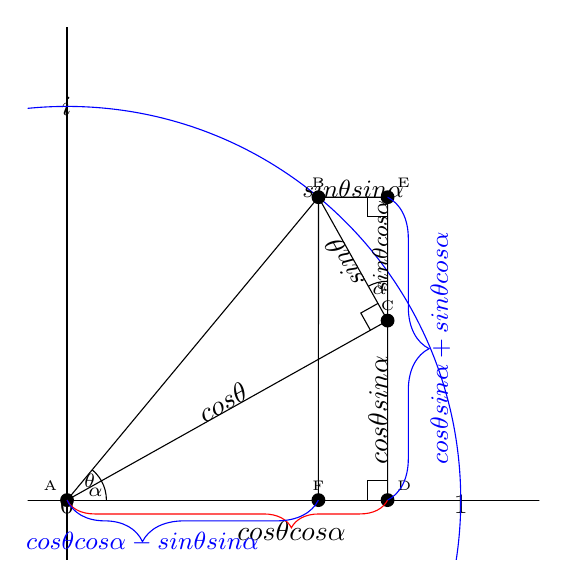
\begin{tikzpicture} [scale=5, rotate=0]
\def\baseangle{117};
\def\angleA{0.25*\baseangle};
\def\angleB{0.18*\baseangle};
\def\myvalue{0.1};
\def\circsiz{0.5pt};
%\clip (-1.5,-1.5) rectangle (1.5,1.5);
\clip (-.1,-.15) rectangle (1.2,1.2);
\draw[black,->] (-2,0) -- (2,0);
\foreach \x in {-1,...,1}
\draw[xshift=\x cm] (0pt,-1pt) -- (0pt,1pt) node[anchor=north] {$\x$};
\draw[black,-] (0,-2) -- (0,2);
\foreach \y in {-1}
\draw[yshift=\y cm] (-1pt,0pt) -- (1pt,0pt) node[anchor=east] {$-i$};
\foreach \y in {1}
\draw[yshift=\y cm] (-1pt,0pt) -- (1pt,0pt) node[anchor=east] {$i$};
\coordinate (A) at (0,0);
\coordinate (Z) at (1,0);
\path [name path=lineA, rotate=\angleA] (0,0) -- (1.1,0);
\path [name path=lineB, rotate=\angleA+\angleB] (0,0) -- (1.1,0);
\node (W) [blue, name path=circle,draw,circle through=(Z)] at (A) {};
\path  [name intersections={of=lineA and circle, by=Y}] (0,0) -- (Y);
\path  [name intersections={of=lineB and circle, by=B}] (0,0) -- (A);
\path [name path=xaxis] (-1.1,0) -- (1.1,0);
\path [name path=yaxis] (0,-1.1) -- (0,1.1);
\path [name path=b-a-sect, rotate=\angleA] (B) -- +(0,-1.1);
\path [name path=b-horiz] (B) -- +(1.1,0);
\path [name path=a-x-sect] (A) -- +(0,-1.1);
\path  [name intersections={of=lineA and b-a-sect, by=C}] (0,0) -- (C);
\path  [name intersections={of=xaxis and a-x-sect, by=X}] (0,0) -- (X);
\path [name path=c-x-sect] (C) -- +(0,-1.1) -- +(0,+2.2);
\path  [name intersections={of=xaxis and c-x-sect, by=D}] (C) -- (D);
\path  [name intersections={of=b-horiz and c-x-sect, by=E}] (C) -- (E);
\path [name path=bdrop] (B) -- +(0,-1.1);
\path  [name intersections={of=xaxis and bdrop, by=F}] (B) -- (F);
\fill [black] (A) circle (\circsiz) node [anchor=south east] {\tiny A};
\fill [black] (B) circle (\circsiz) node [above] {\tiny B};
\fill [black] (C) circle (\circsiz) node [above] {\tiny C};
\fill [black] (D) circle (\circsiz) node [above right] {\tiny D};
\fill [black] (E) circle (\circsiz) node [above right] {\tiny E};
\fill [black] (F) circle (\circsiz) node [above] {\tiny F};
\draw [black] (A) -- (B) -- (C) -- (A);
\draw [black] (C) -- (D);
\draw [black] (B) -- (E);
\draw [black] (C) -- (E);
\draw [black] (B) -- (F);
\draw (0,0) +(\angleA:\myvalue) arc(\angleA:\angleA+\angleB:\myvalue);
\path (0,0) +(\angleA+0.5*\angleB:0.75*\myvalue) node {\scriptsize $\theta$};
\draw (\myvalue,0) arc(0:\angleA:\myvalue);
\path (0,0) +(0.5*\angleA:0.75*\myvalue) node {\scriptsize $\alpha$};
\draw (C) +(90:\myvalue) arc(90:90+\angleA:\myvalue);
\path (C) +(90+.5*\angleA:0.8*\myvalue) node {\scriptsize $\alpha$};
\draw [black] (C) ++(180+\angleA:0.05) -- ++(90+\angleA:0.05) -- +(\angleA:0.05);
\draw [black] (D) ++(180:0.05) -- ++(90:0.05) -- +(0:0.05);
\draw [black] (E) ++(180:0.05) -- ++(90:-0.05) -- +(0:0.05);
\path (B) -- (C) node [midway, rotate=90+\angleA, anchor=base] {$sin\theta$};
\path (A) -- (C) node [midway, rotate=\angleA, anchor=base] {$cos\theta$};
\path (A) -- (D) node [below=4, pos=0.7] {$cos\theta cos\alpha$};
\path (C) -- (D) node [midway, rotate=90, anchor=base] {$cos\theta sin\alpha$};
\path (C) -- (E) node [pos=0.6,  rotate=90, anchor=base] {\footnotesize $sin\theta cos\alpha$};
\path (B) -- (E) node [midway, anchor=base] {\small $sin\theta sin\alpha$};
%\node (V) [blue, name path=circle,draw,circle through=(B)] at (C) {};
\draw [red, decorate,decoration={brace, amplitude=10pt, aspect=0.3}] (D) -- (A) node [black,midway,below=9pt, sloped] {};
\path (F) -- (A) node [blue, below=8, pos=0.7] {\small $cos\theta cos\alpha-sin\theta sin\alpha$};
\draw [blue, decorate,decoration={brace, amplitude=15pt, aspect=0.7}] (F) -- (A) ;
\draw [blue, decorate,decoration={brace, amplitude=15pt}] (E) -- (D) ;
\path (E) -- (D) node [blue, rotate=90, below=12, pos=0.5] {\small $cos\theta sin\alpha+sin\theta cos\alpha$};
%\draw [very thick, black] (A) -- (D) -- (C) --(A);
\end{tikzpicture}
\end{document}

